\documentclass[12pt,a4paper]{article}
\usepackage[utf8]{inputenc}
\usepackage{polski}
\usepackage{geometry}
\usepackage{hyperref}
\usepackage{listings}
\usepackage{xcolor}
\usepackage{graphicx}
\usepackage{float}

\geometry{margin=2.5cm}

% Styl listingów
\lstset{
  basicstyle=\ttfamily\footnotesize,
  keywordstyle=\color{blue},
  commentstyle=\color{green!50!black},
  stringstyle=\color{red},
  showstringspaces=false,
  breaklines=true,
  frame=single
}

\title{Dokumentacja Projektu CryptoLab Mobile}
\author{Agnieszka Ryś}
\date{\today}

\begin{document}
\maketitle
\tableofcontents

\newpage
\section{Cel projektu}
Celem aplikacji \textbf{CryptoLab Mobile} jest edukacja w zakresie kryptografii. 
Aplikacja mobilna pozwala szyfrować i deszyfrować teksty oraz pliki \texttt{.txt}, 
sprawdzać poprawność kluczy oraz eksportować wyniki. 
Aplikacja implementuje zarówno klasyczne szyfry historyczne (Cezara, Vigenère'a, szyfr z kluczem bieżącym), 
jak i nowoczesny standard szyfrowania AES (Advanced Encryption Standard).
Wszystkie algorytmy są implementowane ręcznie, bez użycia gotowych bibliotek kryptograficznych, 
co pozwala na głębsze zrozumienie ich działania.

\section{Podstawy kryptografii klasycznej}

\subsection*{Wprowadzenie}
Kryptografia to dziedzina zajmująca się ochroną informacji poprzez jej przekształcanie w formę nieczytelną dla osób nieuprawnionych. 
Jej historia sięga starożytności, gdzie stosowano proste metody szyfrowania, znane obecnie jako \textbf{kryptografia klasyczna}. 
Celem było zapewnienie poufności korespondencji wojskowej, dyplomatycznej czy handlowej. 

\subsection{Kryptografia symetryczna}
W kryptografii symetrycznej ten sam klucz służy zarówno do szyfrowania, jak i deszyfrowania wiadomości. 
Najważniejsze cechy:
\begin{itemize}
    \item wysoka szybkość działania,
    \item konieczność bezpiecznej wymiany klucza,
    \item podatność na ataki brute-force przy krótkich kluczach.
\end{itemize}

\subsection{Przykłady szyfrów klasycznych}
\begin{itemize}
    \item \textbf{Szyfr Cezara} -- przesunięcie liter alfabetu o stałą liczbę pozycji,
    \item \textbf{Szyfr Vigenère'a} -- wieloalfabetyczny szyfr wykorzystujący słowo-klucz,
    \item \textbf{Szyfr z kluczem bieżącym} -- rozwinięcie Vigenère'a z długim kluczem tekstowym,
    \item \textbf{Szyfr podstawieniowy (monoalfabetyczny)} -- każdej literze alfabetu przypisana jest inna litera,
    \item \textbf{Szyfr Playfair} -- operujący na parach liter,
    \item \textbf{Szyfr transpozycyjny} -- zmienia kolejność znaków w wiadomości.
\end{itemize}

\subsection{Znaczenie w edukacji}
Choć współcześnie klasyczne szyfry nie zapewniają realnego bezpieczeństwa, 
stanowią doskonałe narzędzie dydaktyczne. 
Pozwalają zrozumieć podstawowe pojęcia kryptografii, takie jak:
\begin{itemize}
    \item \textbf{klucz} -- parametr definiujący szyfrowanie,
    \item \textbf{przestrzeń kluczy} -- zbiór możliwych wartości klucza,
    \item \textbf{analiza częstości} -- klasyczna metoda łamania szyfrów,
    \item \textbf{brute-force} -- przeszukiwanie wszystkich możliwych kluczy.
\end{itemize}

\subsection{Nowoczesna kryptografia symetryczna -- AES}
Aplikacja CryptoLab zawiera również implementację \textbf{AES (Advanced Encryption Standard)}, 
który jest standardem współczesnego szyfrowania symetrycznego. 
W przeciwieństwie do szyfrów klasycznych, AES:
\begin{itemize}
    \item jest szyfrem \textbf{blokowym} (operuje na blokach 128 bitów),
    \item wykorzystuje złożone operacje matematyczne (S-Box, MixColumns, ShiftRows),
    \item oferuje różne długości kluczy (128, 192, 256 bitów),
    \item obsługuje różne tryby pracy (ECB, CBC, CTR),
    \item jest odporny na wszystkie znane praktyczne ataki kryptograficzne.
\end{itemize}

Dzięki implementacji zarówno szyfrów klasycznych, jak i nowoczesnego AES, 
użytkownicy mogą porównać podejścia historyczne z obecnie stosowanymi rozwiązaniami 
i zrozumieć ewolucję kryptografii.

\section{Miejsce szyfru Cezara}
Szyfr Cezara należy do najprostszych szyfrów podstawieniowych. 
Choć jego bezpieczeństwo jest znikome, odgrywa on kluczową rolę w nauczaniu, 
ponieważ wprowadza intuicyjnie pojęcia klucza, szyfrowania i deszyfrowania. 
CryptoLab wykorzystuje go jako \textbf{pierwszy krok} w implementacji i analizie algorytmów kryptograficznych.


\section{Technologie wykorzystane w projekcie}

\begin{description}
    \item[\textbf{React Native + Expo}] 
    Główna platforma wykorzystana do tworzenia aplikacji mobilnych. 
    React Native umożliwia budowanie natywnych aplikacji na systemy Android i iOS, wykorzystując składnię zbliżoną do Reacta. 
    Expo zostało użyte jako narzędzie wspierające proces developmentu – upraszcza konfigurację środowiska, przyspiesza testowanie na urządzeniach mobilnych i zapewnia dostęp do bogatego ekosystemu bibliotek.

    \item[\textbf{TypeScript}] 
    Nadzbiór JavaScriptu wprowadzający system typów. 
    Zastosowanie TypeScriptu pozwoliło na: 
    \begin{itemize}
        \item wcześniejsze wykrywanie błędów podczas kompilacji,
        \item lepszą kontrolę nad strukturą danych i interfejsami,
        \item zwiększoną czytelność oraz przewidywalność kodu,
    \end{itemize}

    \item[\textbf{Expo Document Picker, File System, Vector Icons}] 
    Dodatkowe biblioteki środowiska Expo: 
    \begin{itemize}
        \item \texttt{expo-document-picker} – umożliwia wybór plików z pamięci urządzenia, 
        \item \texttt{expo-file-system} – zapewnia dostęp do systemu plików (zapisywanie, odczyt, usuwanie plików),
        \item \texttt{expo-vector-icons} – biblioteka ikon pozwalająca wzbogacić interfejs użytkownika.
    \end{itemize}

    \item[\textbf{Git}] 
    System kontroli wersji użyty do zarządzania historią kodu. 
    Pozwolił na prowadzenie szczegółowego changelogu, śledzenie postępów w projekcie oraz łatwe zarządzanie zmianami w kodzie źródłowym.

    \item[\textbf{LaTeX}] 
    System składu tekstu wykorzystany do przygotowania dokumentacji. 
    Umożliwia on: 
    \begin{itemize}
        \item zachowanie spójności formatowania,
        \item wygodne dodawanie fragmentów kodu źródłowego i zrzutów ekranu,
        \item automatyczne generowanie spisów treści i numeracji.
    \end{itemize}
\end{description}

\newpage

\section{Architektura systemu}

\subsection{Wzorzec projektowy}
Aplikacja wykorzystuje \textbf{Strategy Pattern} dla algorytmów kryptograficznych. 
Każdy algorytm dziedziczy z klasy abstrakcyjnej \texttt{CryptographicAlgorithm} i implementuje metody:
\begin{itemize}
    \item \texttt{encrypt(plaintext, key)} -- szyfruje tekst,
    \item \texttt{decrypt(ciphertext, key)} -- deszyfruje tekst,
    \item \texttt{validateKey(key)} -- sprawdza poprawność klucza,
    \item \texttt{getKeyRequirements()} -- zwraca opis wymagań dla klucza.
\end{itemize}

Wszystkie algorytmy zarejestrowane są w \texttt{AlgorithmRegistry} (Singleton Pattern), 
co umożliwia łatwe dodawanie nowych szyfrów bez modyfikacji głównej aplikacji.

\subsection{Komponenty główne}
\begin{itemize}
    \item \textbf{App.tsx} -- główny komponent aplikacji, obsługuje interfejs użytkownika,
    \item \textbf{AlgorithmSidebar.tsx} -- boczny panel z listą dostępnych algorytmów,
    \item \textbf{AlgorithmRegistry.ts} -- rejestr i zarządzanie algorytmami,
    \item \textbf{CryptographicAlgorithm.ts} -- klasa bazowa dla wszystkich algorytmów,
    \item \textbf{fileUtils.ts} -- funkcje do obsługi operacji na plikach.
\end{itemize}

\section{Struktura projektu}
\begin{lstlisting}
crypto-lab-mobile/
├── App.tsx                          (glowny komponent)
├── package.json                     (zalezności projektu)
├── tsconfig.json                    (konfiguracja TypeScriptu)
├── app.json                         (konfiguracja Expo)
├── src/
│   ├── algorithms/
│   │   ├── CryptographicAlgorithm.ts   (klasa bazowa)
│   │   ├── CaesarCipher.ts             (szyfr Cezara)
│   │   ├── VigenereCipher.ts           (szyfr Vigenere'a)
│   │   ├── RunningKeyCipher.ts         (szyfr z kluczem biezacym)
│   │   ├── AESCipher.ts                (szyfr AES)
│   │   └── AlgorithmRegistry.ts        (rejestr algorytmow)
│   ├── components/
│   │   └── AlgorithmSidebar.tsx        (panel z algorytmami)
│   └── utils/
│       └── fileUtils.ts                (obsluga plikow)
└── assets/                          (zasoby graficzne)
\end{lstlisting}
\section{Implementacja szyfru Cezara}
\subsection{Podstawy}
Szyfr Cezara to prosty szyfr monoalfabetyczny, w którym litery przesuwane są o wartość klucza $k$. 
Przestrzeń kluczy obejmuje wartości $1$--$25$. 
Metoda jest podatna na ataki brute-force i analizę częstotliwości.

\subsection{Model matematyczny}
\begin{itemize}
    \item Szyfrowanie: $E_k(x) = (x + k) \bmod 26$,
    \item Deszyfrowanie: $D_k(x) = (x - k) \bmod 26$.
\end{itemize}

\subsection{Cechy implementacji}
\begin{itemize}
    \item Obsługuje zarówno wielkie jak i małe litery,
    \item Znaki niebędące literami pozostają bez zmian,
    \item Klucz musi być liczbą całkowitą z zakresu 1--25,
    \item Walidacja klucza zwraca szczegółową informację o błędach.
\end{itemize}

\newpage
\section{Implementacja szyfru Vigenère'a}

\subsection{Historia i znaczenie}
Szyfr Vigenère'a został opracowany w XVI wieku przez Blaise de Vigenère'a. 
Przez długi czas uważany był za niezniszczalny (\textit{le chiffre indéchiffrable}) 
aż do jego przełamania przez Charles'a Babbage'a w XIX wieku.

\subsection{Podstawy}
Szyfr Vigenère'a to szyfr \textbf{polialfabetyczny}, który wykorzystuje słowo-klucz 
do generowania serii przesunięć. W przeciwieństwie do szyfru Cezara, 
każda litera tekstu może być szyfrowana z innym przesunięciem.

\subsection{Model matematyczny}
\begin{itemize}
    \item Szyfrowanie: $E_{k}(x_i) = (x_i + k_{i \bmod |k|}) \bmod 26$,
    \item Deszyfrowanie: $D_{k}(y_i) = (y_i - k_{i \bmod |k|}) \bmod 26$,
    \item gdzie $k$ to słowo-klucz, a $|k|$ to jego długość.
\end{itemize}

\subsection{Przykład działania}
\begin{center}
\begin{tabular}{|c|c|c|c|c|c|c|}
\hline
Tekst jawny & A & T & T & A & C & K \\
\hline
Klucz & L & E & M & O & N & L \\
\hline
Przesunięcia & +11 & +4 & +12 & +14 & +13 & +11 \\
\hline
Tekst zaszyfrowany & L & X & F & O & P & V \\
\hline
\end{tabular}
\end{center}

\subsection{Cechy implementacji}
\begin{itemize}
    \item Klucz może zawierać tylko litery (A-Z, a-z),
    \item Klucz nie może być pusty,
    \item Znaki niebędące literami w tekście źródłowym są przepisywane bez zmian,
    \item Klucz automatycznie się powtarza dla długich tekstów,
    \item Obsługuje zarówno wielkie jak i małe litery w tekście.
\end{itemize}
\newpage
\section{Implementacja szyfru z kluczem bieżącym}

\subsection{Historia i zastosowanie}
Szyfr z kluczem bieżącym (Running Key Cipher) to rozwinięcie szyfru Vigenère'a. 
Zamiast krótko słowa, wykorzystuje on klucz o długości co najmniej równej długości tekstu. 
Gdy klucz jest naprawdę losowy i będzie użyty tylko raz, szyfr ten jest teoretycznie nie do złamania 
(jest to wariant szyfru jednorazowego -- \textit{One-Time Pad}).

\subsection{Podstawy}
Algorytm jest w zasadzie identyczny z szyfrem Vigenère'a, ale z istotną różnicą: 
klucz powinien być znacznie dłuższy niż tekst. W praktyce zastosowania edukacyjnego 
aplikacja automatycznie generuje klucz z tekstu Lorem Ipsum.

\subsection{Model matematyczny}
\begin{itemize}
    \item Szyfrowanie: $E_{k}(x_i) = (x_i + k_i) \bmod 26$,
    \item Deszyfrowanie: $D_{k}(y_i) = (y_i - k_i) \bmod 26$,
    \item gdzie $|k| \geq |x|$ (klucz jest co najmniej tak długi jak tekst).
\end{itemize}

\subsection{Cechy implementacji}
\begin{itemize}
    \item Klucz może zawierać litery i spacje,
    \item Klucz musi zawierać co najmniej 5 liter,
    \item Aplikacja automatycznie generuje losowy klucz na bazie Lorem Ipsum,
    \item Zaszyfrowany tekst zawiera klucz w formacie: \texttt{<klucz>::<tekst\_zaszyfrowany>},
    \item Deszyfrowanie wymaga podania tekstu w poprawnym formacie.
\end{itemize}

\subsection{Bezpieczeństwo}
\begin{itemize}
    \item Gdy klucz jest losowy i używany tylko raz, szyfr jest teoretycznie bezpieczny,
    \item Słaba strona: jeśli klucz jest krótszy niż tekst, powtarza się i traci bezpieczeństwo,
    \item W aplikacji edukacyjne klucz jest generowany automatycznie i przechowywany w wynikach.
\end{itemize}

\newpage
\section{Implementacja szyfru AES}

\subsection{Historia i znaczenie}
AES (Advanced Encryption Standard) to symetryczny szyfr blokowy, który w 2001 roku został wybrany przez NIST (National Institute of Standards and Technology) jako następca przestarzałego algorytmu DES. 
Został opracowany przez belgijskich kryptografów Joana Daemena i Vincenta Rijmena pod nazwą \textit{Rijndael}. 
AES jest obecnie najpowszechniej stosowanym szyfrem symetrycznym na świecie -- chroni dane w protokołach SSL/TLS, systemach bankowych, szyfrowanych dyskach i wielu innych zastosowaniach.

\subsection{Podstawy}
AES to szyfr \textbf{blokowy}, który operuje na blokach danych o długości 128 bitów (16 bajtów). 
W przeciwieństwie do szyfrów klasycznych, AES wykorzystuje skomplikowane operacje matematyczne na macierzach bajtów, 
w tym podstawienia (S-Box), permutacje, mieszanie kolumn i dodawanie klucza rundowego.

\subsection{Warianty AES}
AES występuje w trzech wariantach, różniących się długością klucza:
\begin{itemize}
    \item \textbf{AES-128} -- klucz 128-bitowy (32 znaki hex), 10 rund szyfrowania,
    \item \textbf{AES-192} -- klucz 192-bitowy (48 znaków hex), 12 rund szyfrowania,
    \item \textbf{AES-256} -- klucz 256-bitowy (64 znaki hex), 14 rund szyfrowania.
\end{itemize}

Im dłuższy klucz, tym wyższe bezpieczeństwo, ale także nieznacznie wolniejsze działanie.
\begin{figure}[H]
    \centering
    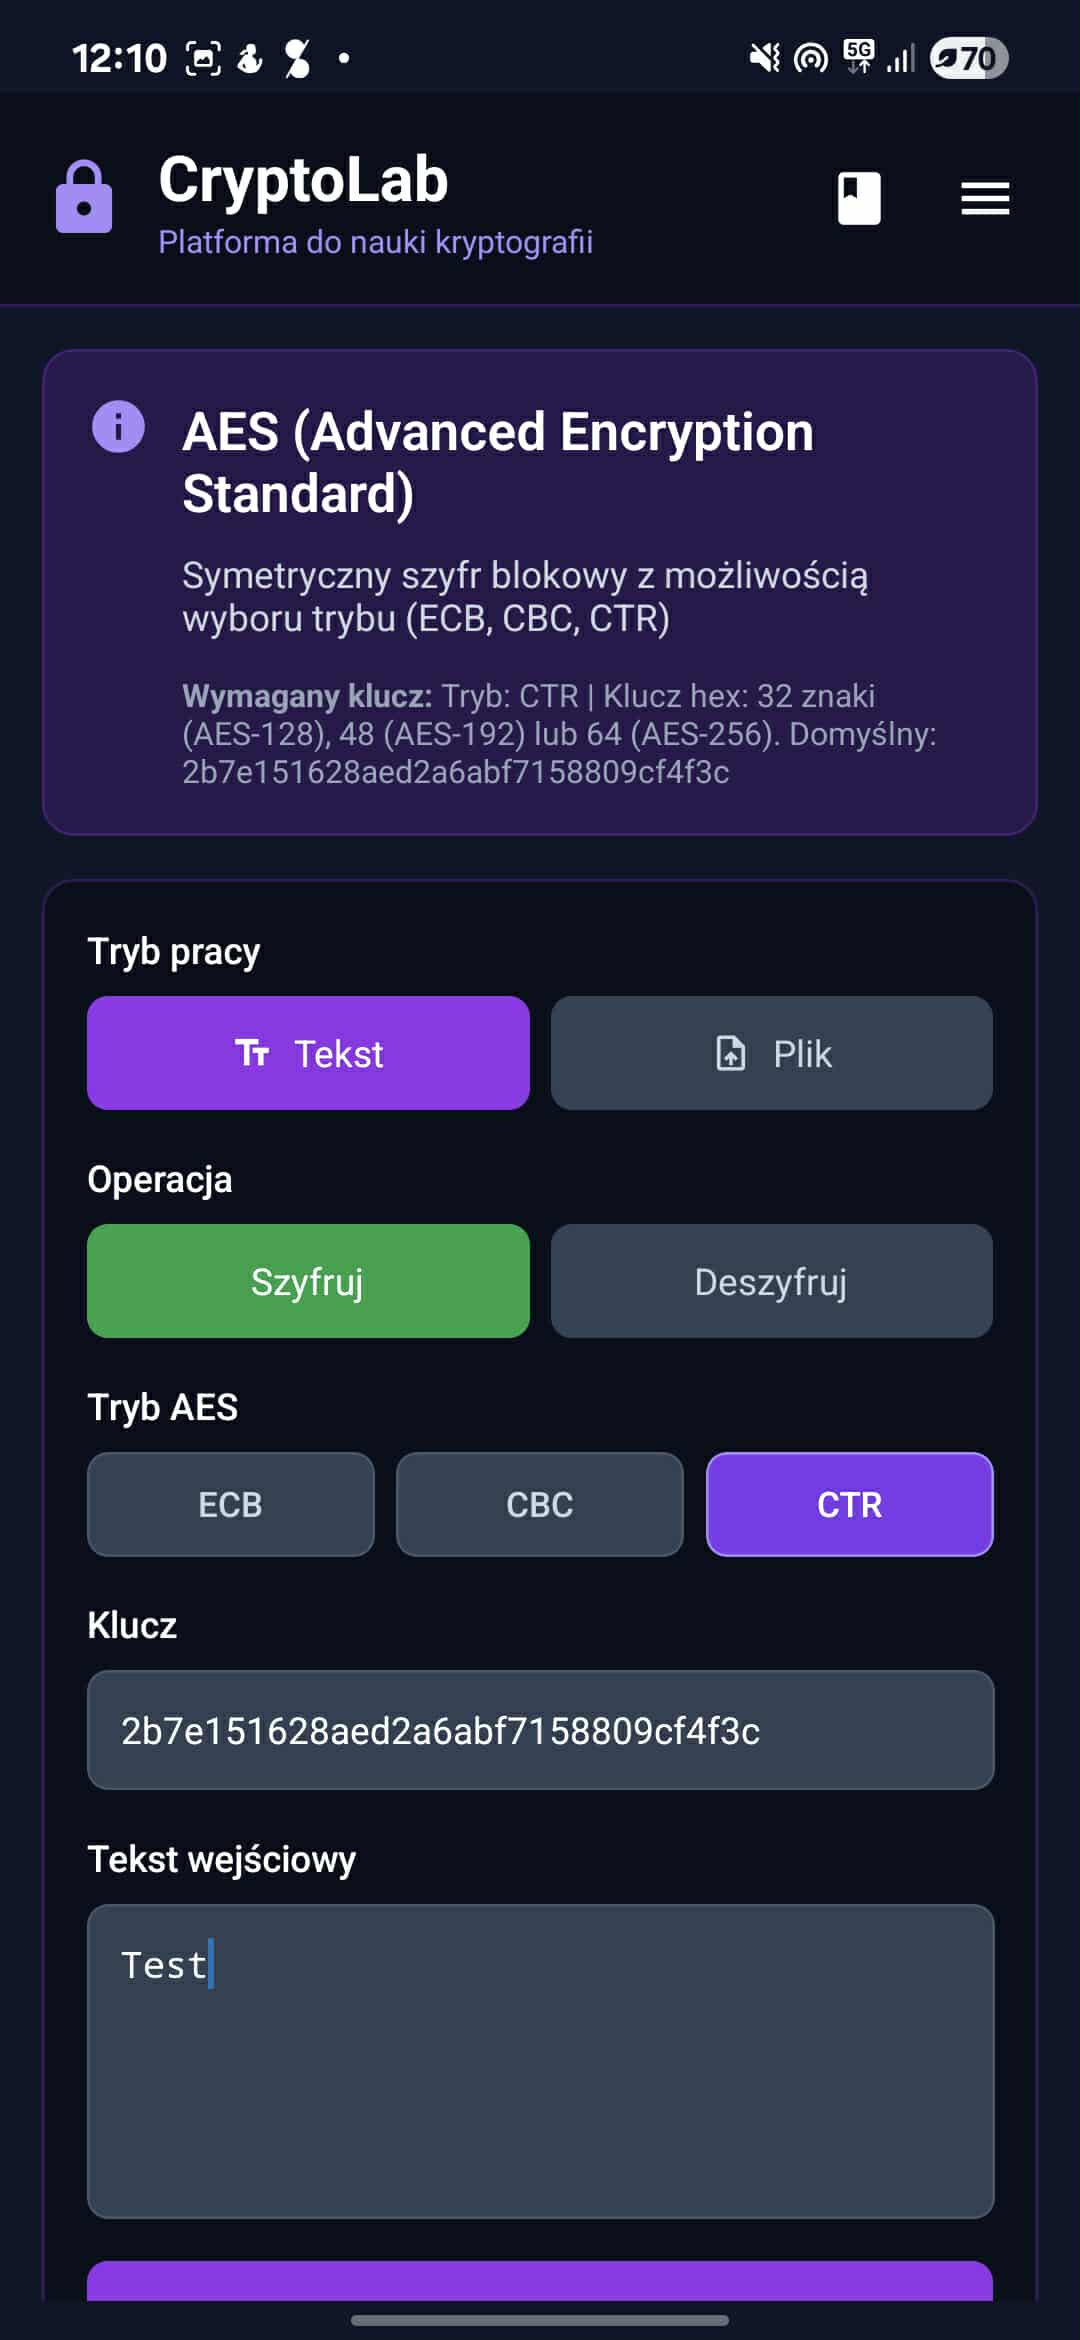
\includegraphics[width=0.3\textwidth]{img/strona_glownaAES.jpg}
    \caption{Strona główna szyfru AES w aplikacji CryptoLab}
    \label{fig:aes_main}
\end{figure}
Rysunek \ref{fig:aes_main} przedstawia interfejs użytkownika aplikacji CryptoLab Mobile dla szyfru AES.
\subsection{Tryby pracy AES}
Szyfr blokowy wymaga określenia \textbf{trybu pracy}, który definiuje sposób szyfrowania wielu bloków danych:

\begin{description}
    \item[\textbf{ECB (Electronic Codebook)}] 
    Najprostszy tryb -- każdy blok szyfrowany jest niezależnie tym samym kluczem. 
    \textbf{Niezalecany} w praktyce, ponieważ identyczne bloki tekstu jawnego dają identyczne bloki szyfrogramu, 
    co może ujawnić wzorce w danych.
    \begin{figure}
        \centering
        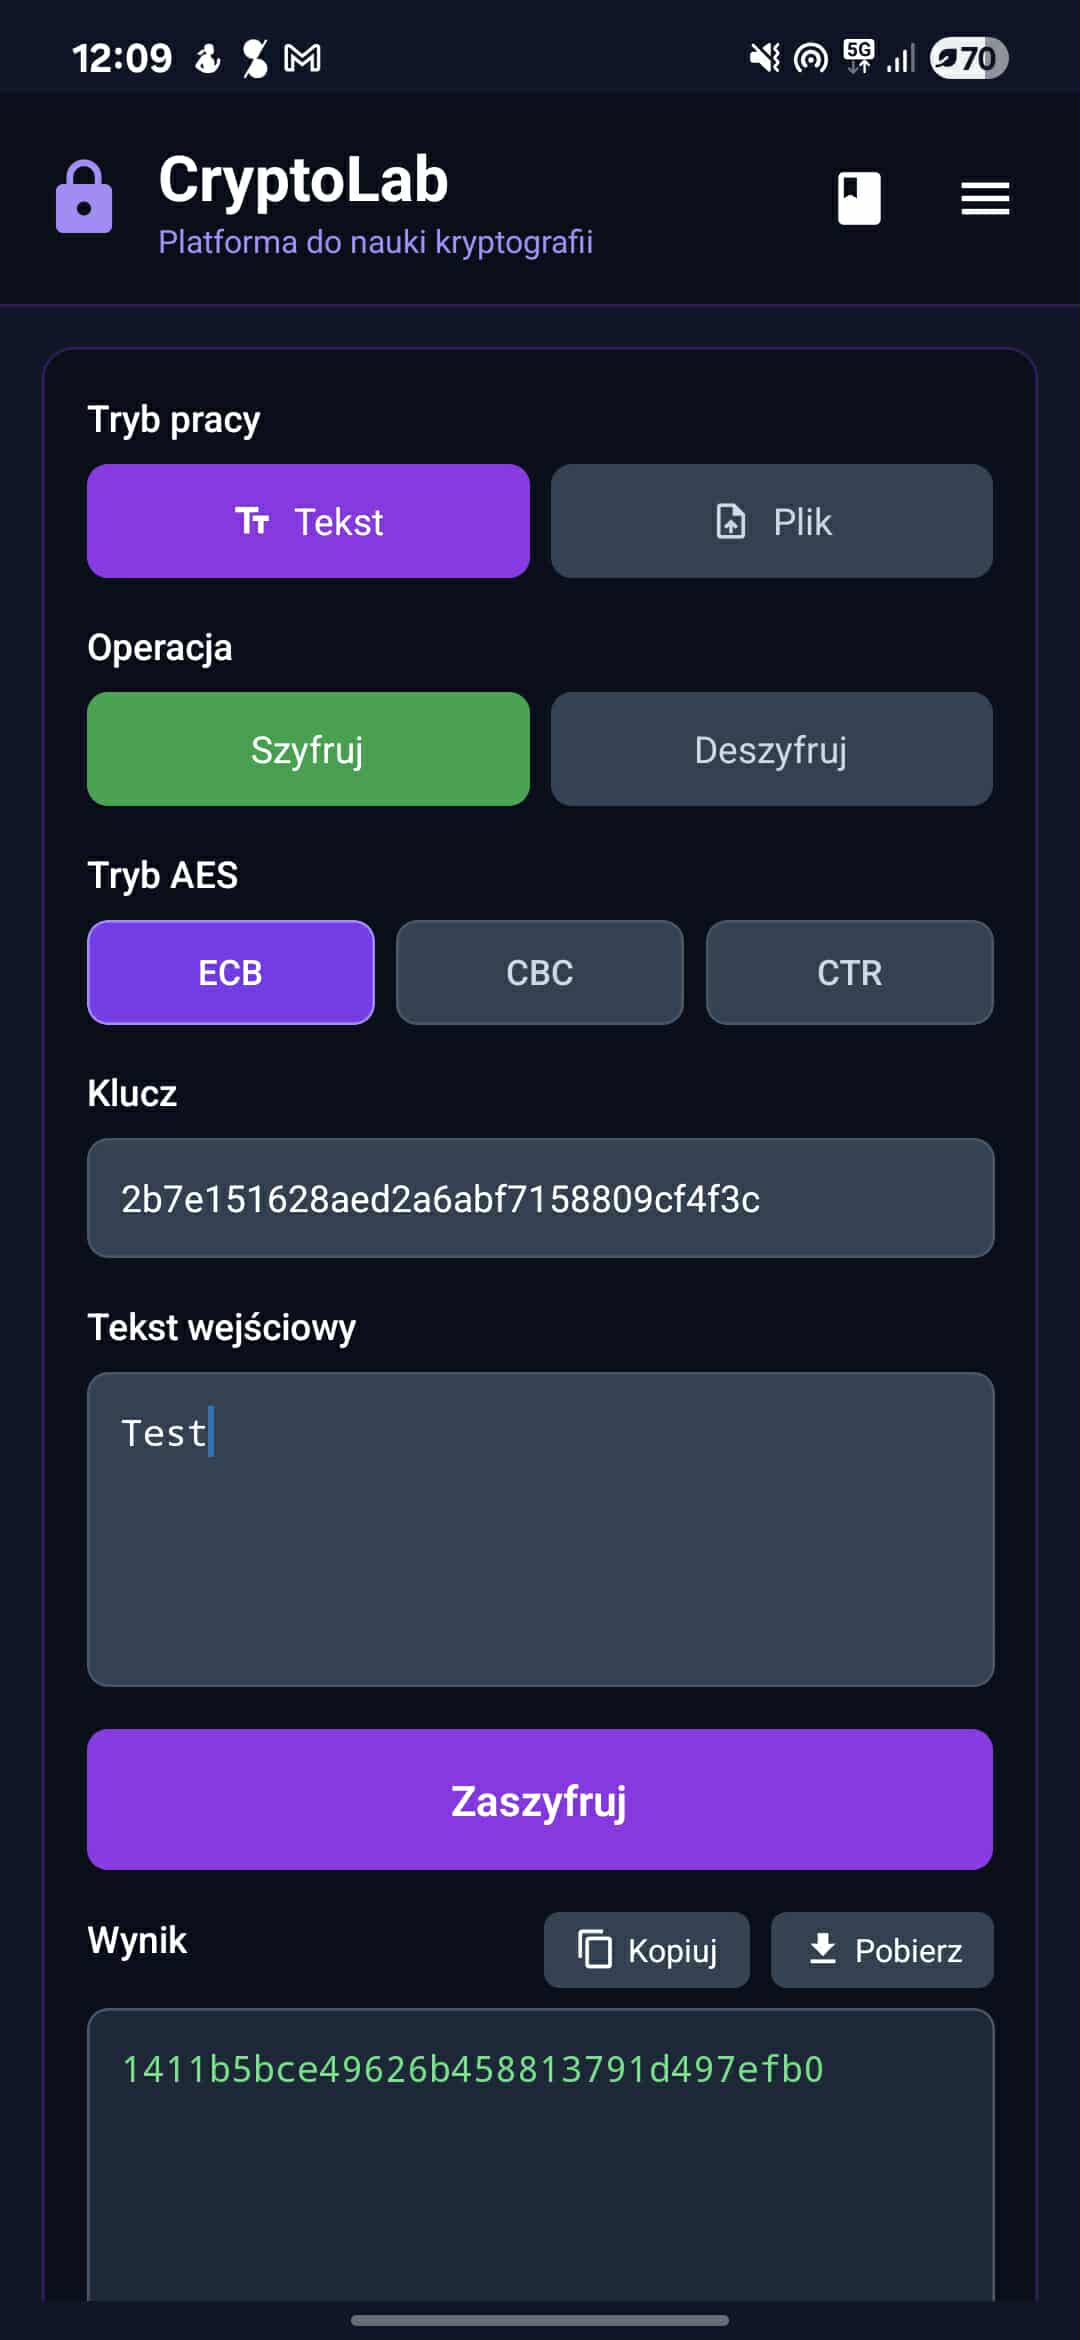
\includegraphics[width=0.3\textwidth]{img/ECB.jpg}
        \caption{Tryb ECB w szyfrze AES}
        \label{fig:ecb}
    \end{figure}
    Rysunek \ref{fig:ecb} przedstawia przykładowe szyfrowanie tekstu w trybiie ECB.
    
    \item[\textbf{CBC (Cipher Block Chaining)}] 
    Każdy blok tekstu jawnego jest najpierw XOR-owany z poprzednim blokiem szyfrogramu przed zaszyfrowaniem. 
    Wymaga wektora inicjalizującego (IV). Tryb ten ukrywa wzorce w danych i jest szeroko stosowany.
    \begin{figure}
        \centering
        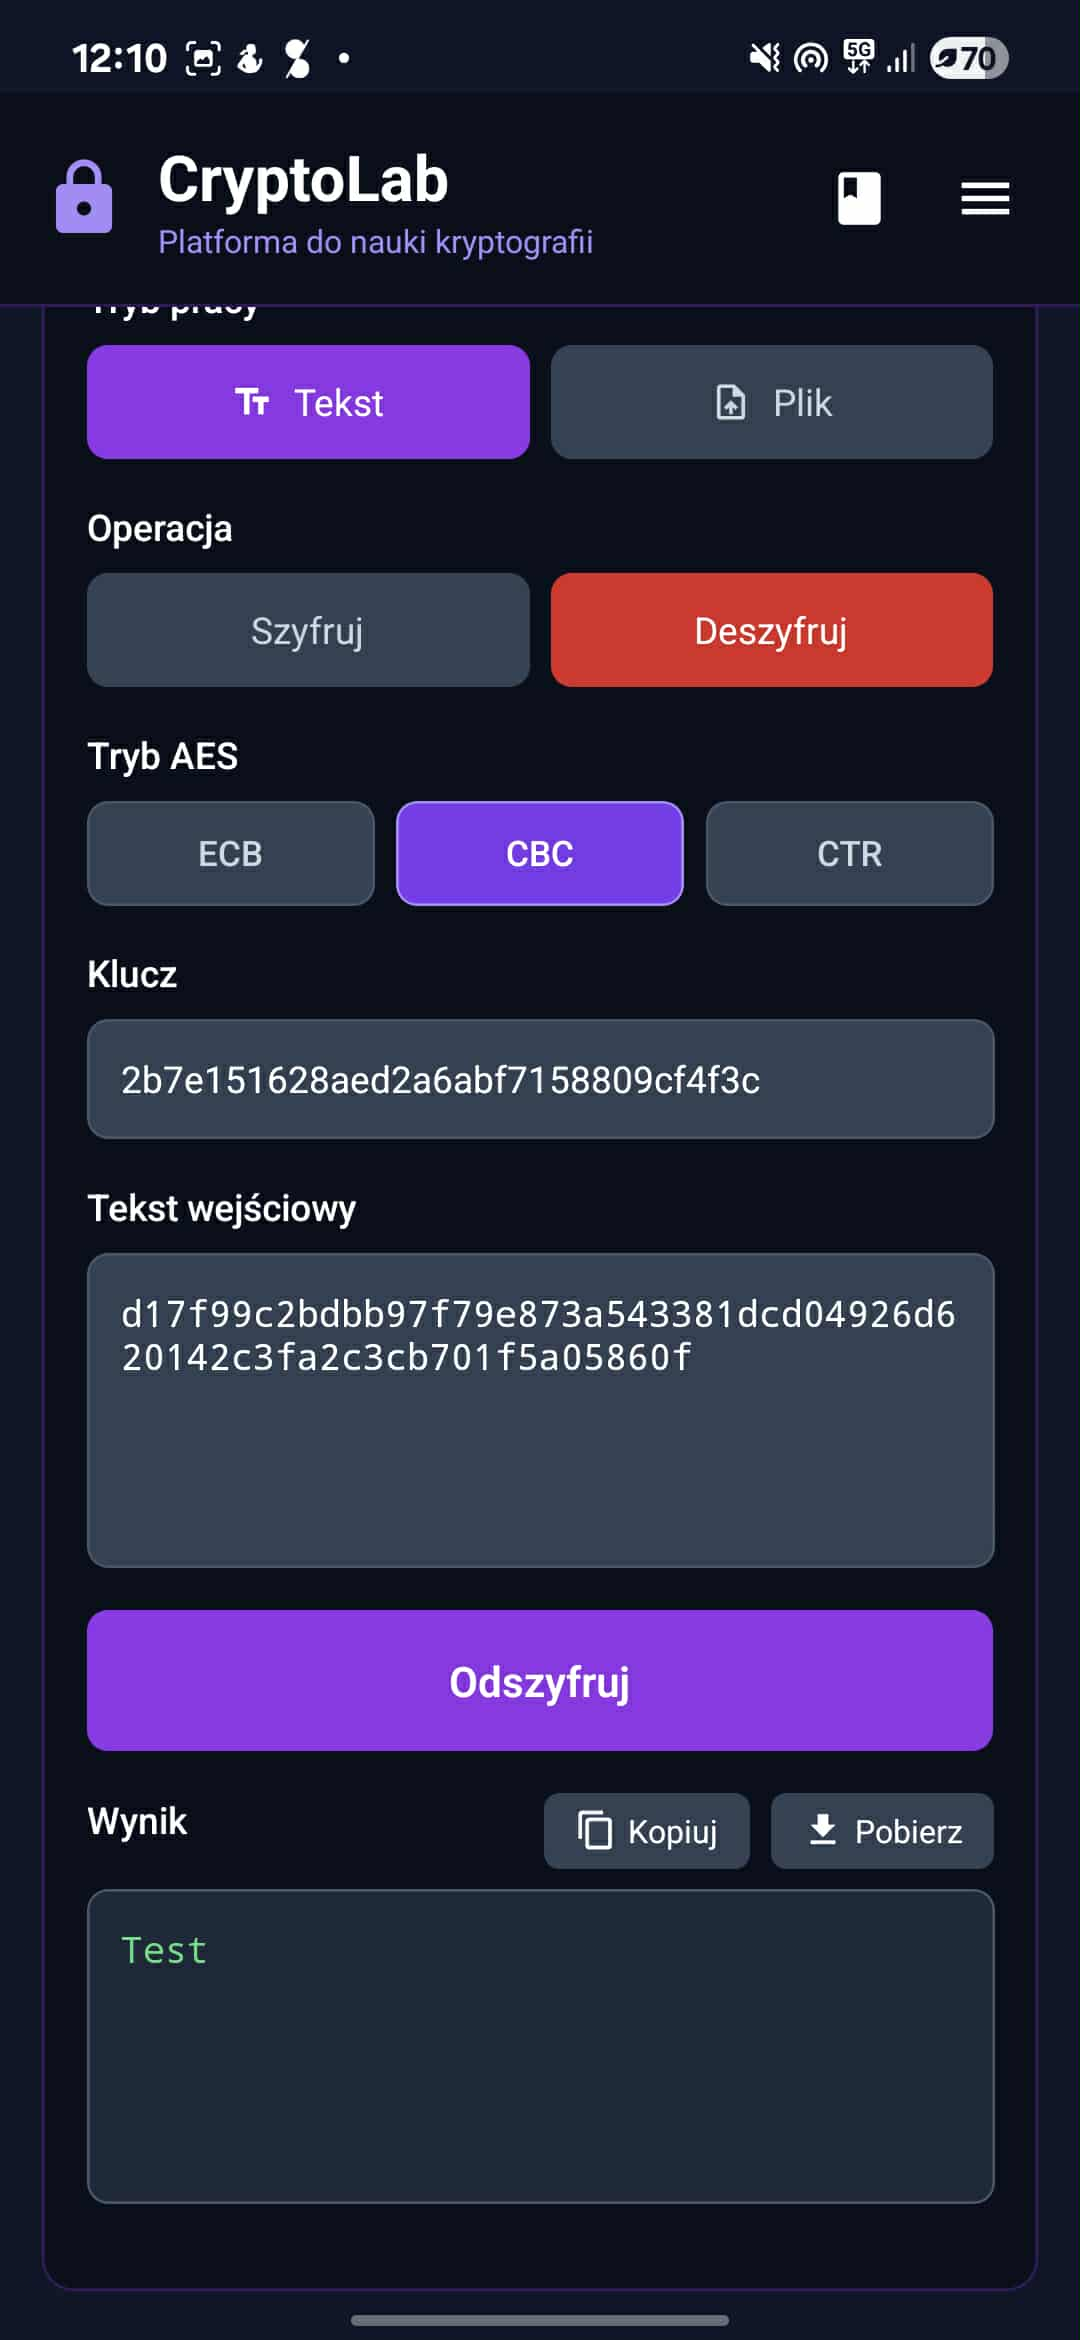
\includegraphics[width=0.3\textwidth]{img/CBC.jpg}
        \caption{Tryb CBC w szyfrze AES}
        \label{fig:cbc}
    \end{figure}
    Rysunek \ref{fig:cbc} przedstawia przykładowe deszyfrowanie tekstu w trybiie CBC.
    \item[\textbf{CTR (Counter Mode)}] 
    Przekształca szyfr blokowy w szyfr strumieniowy. 
    Szyfruje kolejne wartości licznika, a wyniki XOR-uje z blokami tekstu jawnego. 
    Umożliwia równoległe szyfrowanie i deszyfrowanie.
    \begin{figure}
        \centering
        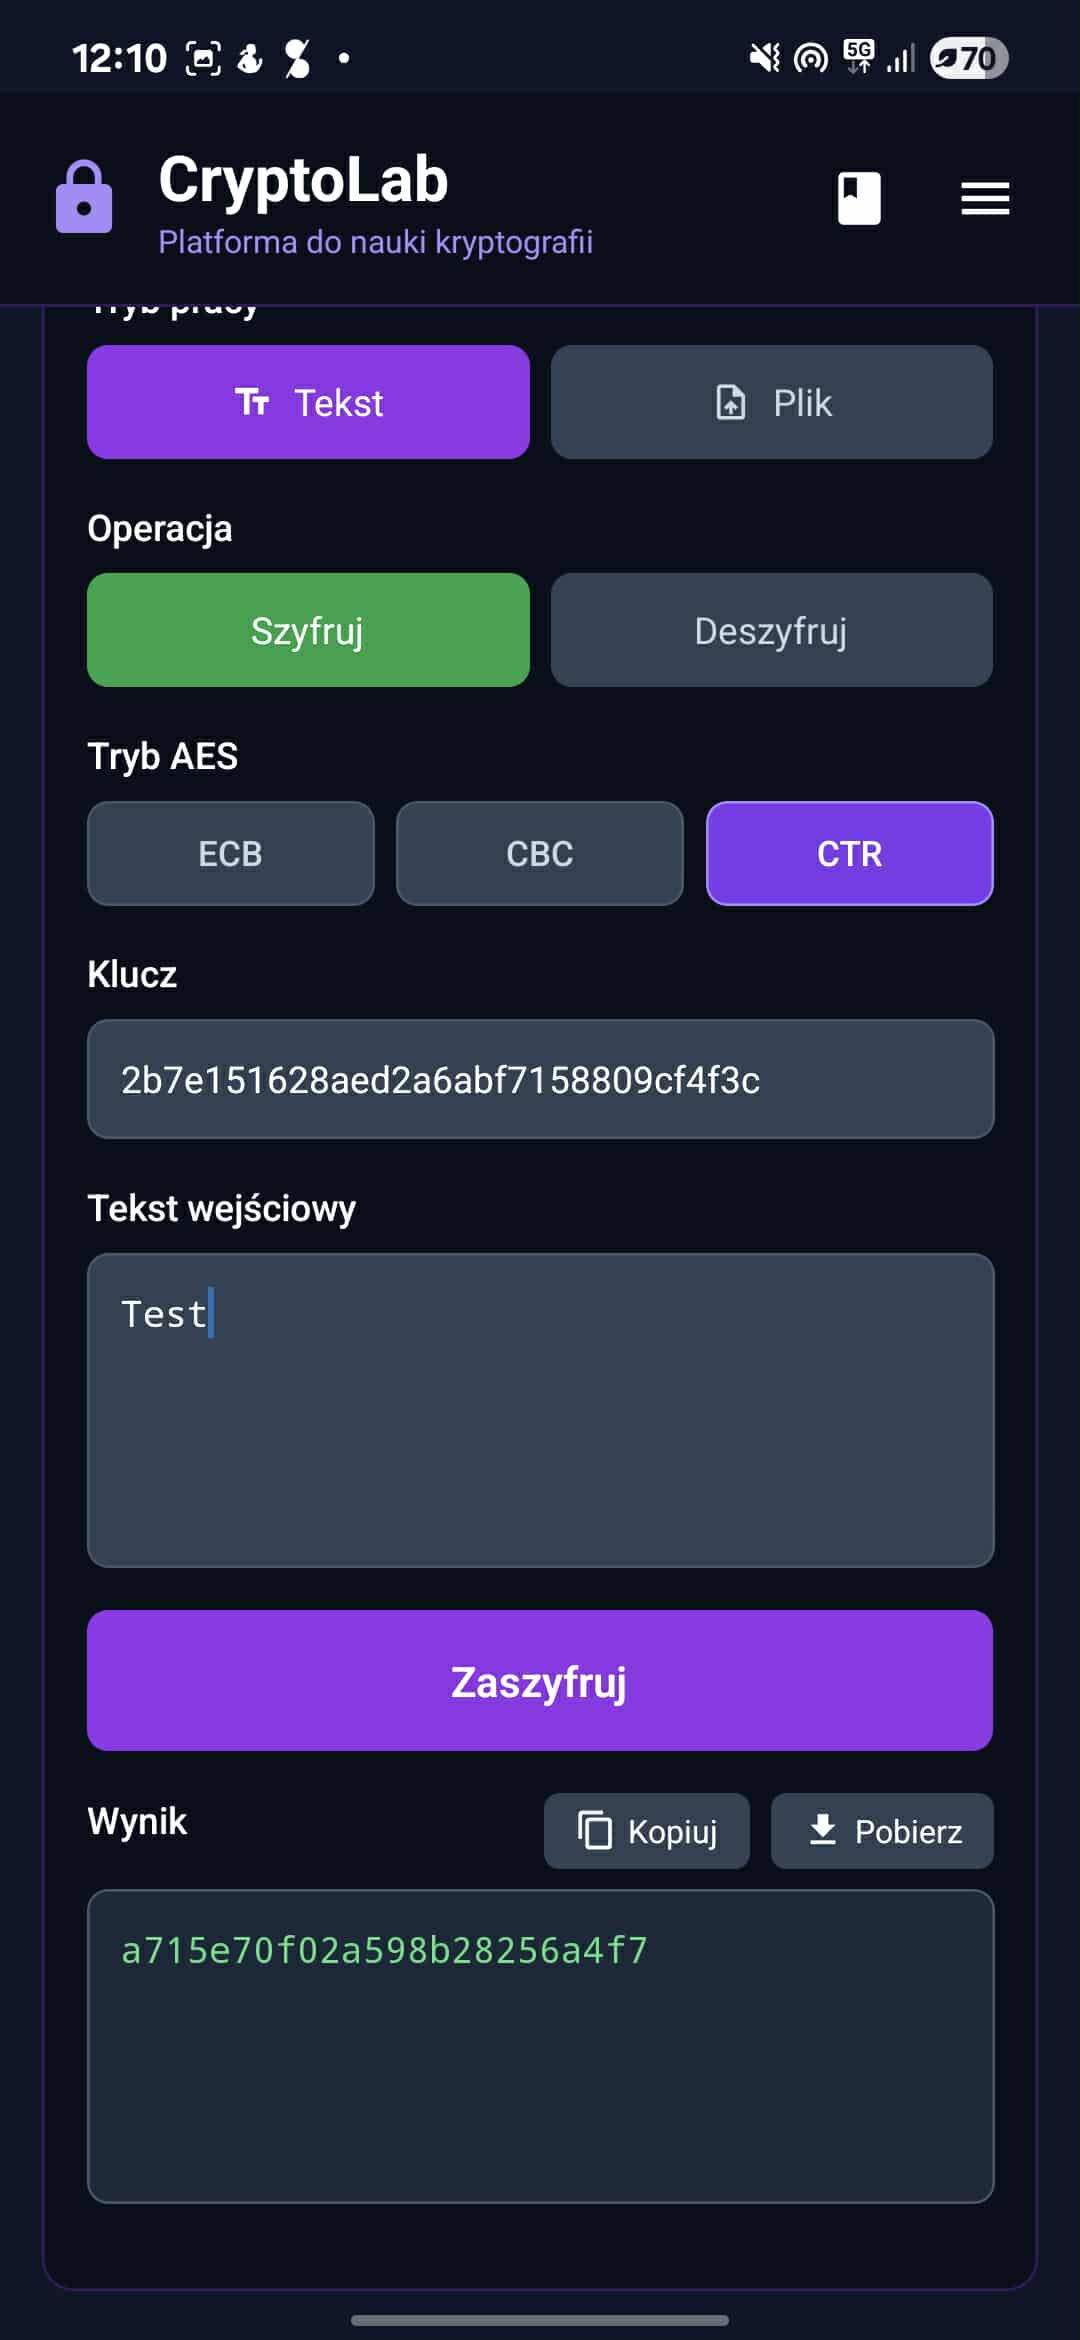
\includegraphics[width=0.3\textwidth]{img/CTR.jpg}
        \caption{Tryb CTR w szyfrze AES}
        \label{fig:ctr}
    \end{figure}
    Rysunek \ref{fig:ctr} przedstawia przykładowe szyfrowanie tekstu w trybiie CTR.
\end{description}

\subsection{Struktura algorytmu AES}
Algorytm AES składa się z następujących kroków (dla każdej rundy):
\begin{enumerate}
    \item \textbf{SubBytes} -- podstawienie bajtów zgodnie z tablicą S-Box,
    \item \textbf{ShiftRows} -- przesunięcie wierszy macierzy stanu,
    \item \textbf{MixColumns} -- mieszanie kolumn macierzy (pomijane w ostatniej rundzie),
    \item \textbf{AddRoundKey} -- dodanie klucza rundowego (operacja XOR).
\end{enumerate}

Przed pierwszą rundą wykonywana jest operacja \texttt{AddRoundKey} z kluczem początkowym.

\subsection{Cechy implementacji}
\begin{itemize}
    \item Obsługuje klucze w formacie szesnastkowym (hex),
    \item Klucz musi mieć długość 32, 48 lub 64 znaki hex (AES-128/192/256),
    \item Domyślny klucz: \texttt{2b7e151628aed2a6abf7158809cf4f3c} (AES-128),
    \item Implementuje trzy tryby pracy: ECB, CBC, CTR,
    \item Używa paddingu PKCS\#7 dla dopełnienia bloków,
    \item Generuje losowy wektor inicjalizujący (IV) dla trybów CBC i CTR,
    \item Wynik szyfrowania zwracany w formacie hex,
    \item Pełna implementacja bez użycia zewnętrznych bibliotek kryptograficznych.
\end{itemize}

\subsection{Bezpieczeństwo}
\begin{itemize}
    \item AES jest uważany za \textbf{kryptograficznie bezpieczny} przy prawidłowym użyciu,
    \item Nie znaleziono praktycznych ataków na pełny AES-128, AES-192 ani AES-256,
    \item Teoretyczne ataki istnieją, ale wymagają zasobów przekraczających możliwości obecnej technologii,
    \item Bezpieczeństwo zależy od:
    \begin{itemize}
        \item wyboru odpowiedniego trybu pracy (CBC lub CTR zamiast ECB),
        \item użycia losowego IV dla trybów CBC i CTR,
        \item odpowiedniej długości klucza (zalecane minimum: AES-128),
        \item bezpiecznego przechowywania i dystrybucji klucza.
    \end{itemize}
\end{itemize}

\subsection{Zastosowania}
AES jest wykorzystywany w:
\begin{itemize}
    \item szyfrowanie połączeń internetowych (HTTPS, SSL/TLS),
    \item pełne szyfrowanie dysków (BitLocker, FileVault),
    \item sieci bezprzewodowe (WPA2, WPA3),
    \item aplikacje bankowe i systemy płatności,
    \item komunikatory szyfrowane (Signal, WhatsApp),
    \item archiwizacja danych (7-Zip, WinRAR z szyfrowaniem AES).
\end{itemize}

\newpage
\section{Wybrane fragmenty kodu}
\subsection{Klasa bazowa algorytmu}
\begin{lstlisting}[language=TypeScript, caption={Klasa abstrakcyjna CryptographicAlgorithm}]
export default class CryptographicAlgorithm {
  name: string;
  description: string;
  category: string;

  encrypt(plaintext: string, key: string): string {
    throw new Error('Metoda encrypt() musi być zaimplementowana');
  }

  decrypt(ciphertext: string, key: string): string {
    throw new Error('Metoda decrypt() musi być zaimplementowana');
  }

  validateKey(key: string): { valid: boolean; error?: string } {
    throw new Error('Metoda validateKey() musi być zaimplementowana');
  }

  getKeyRequirements(): string {
    throw new Error('Metoda getKeyRequirements() musi być zaimplementowana');
  }
}
\end{lstlisting}
\begin{figure}[H]
    \centering
    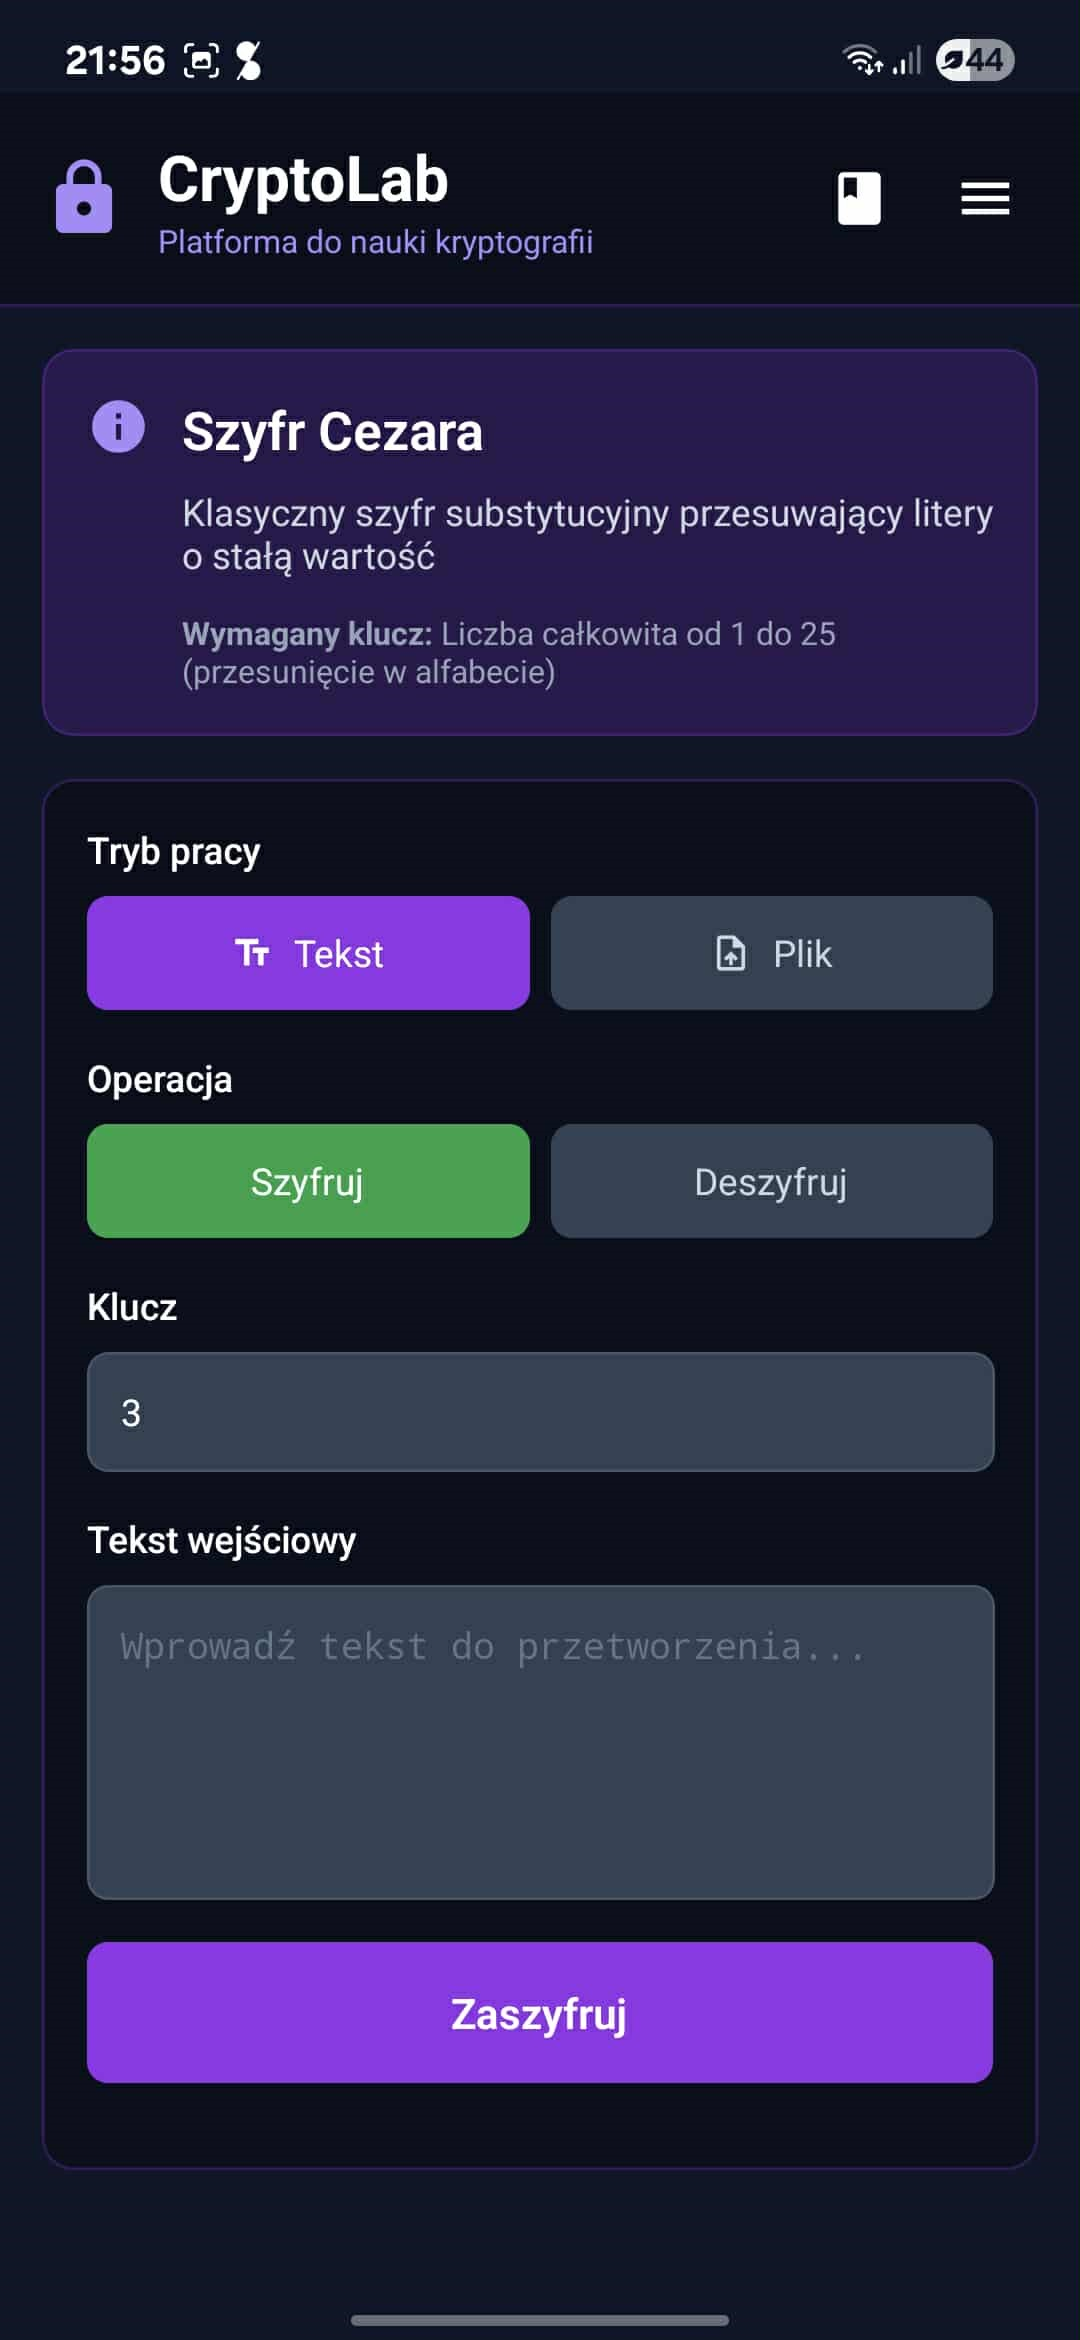
\includegraphics[width=0.3\textwidth]{img/szyfr_cezara.jpg}
    \caption{Ekran główny aplikacji CryptoLab}
    \label{fig:main}
\end{figure}
\begin{figure}[H]
    \centering
    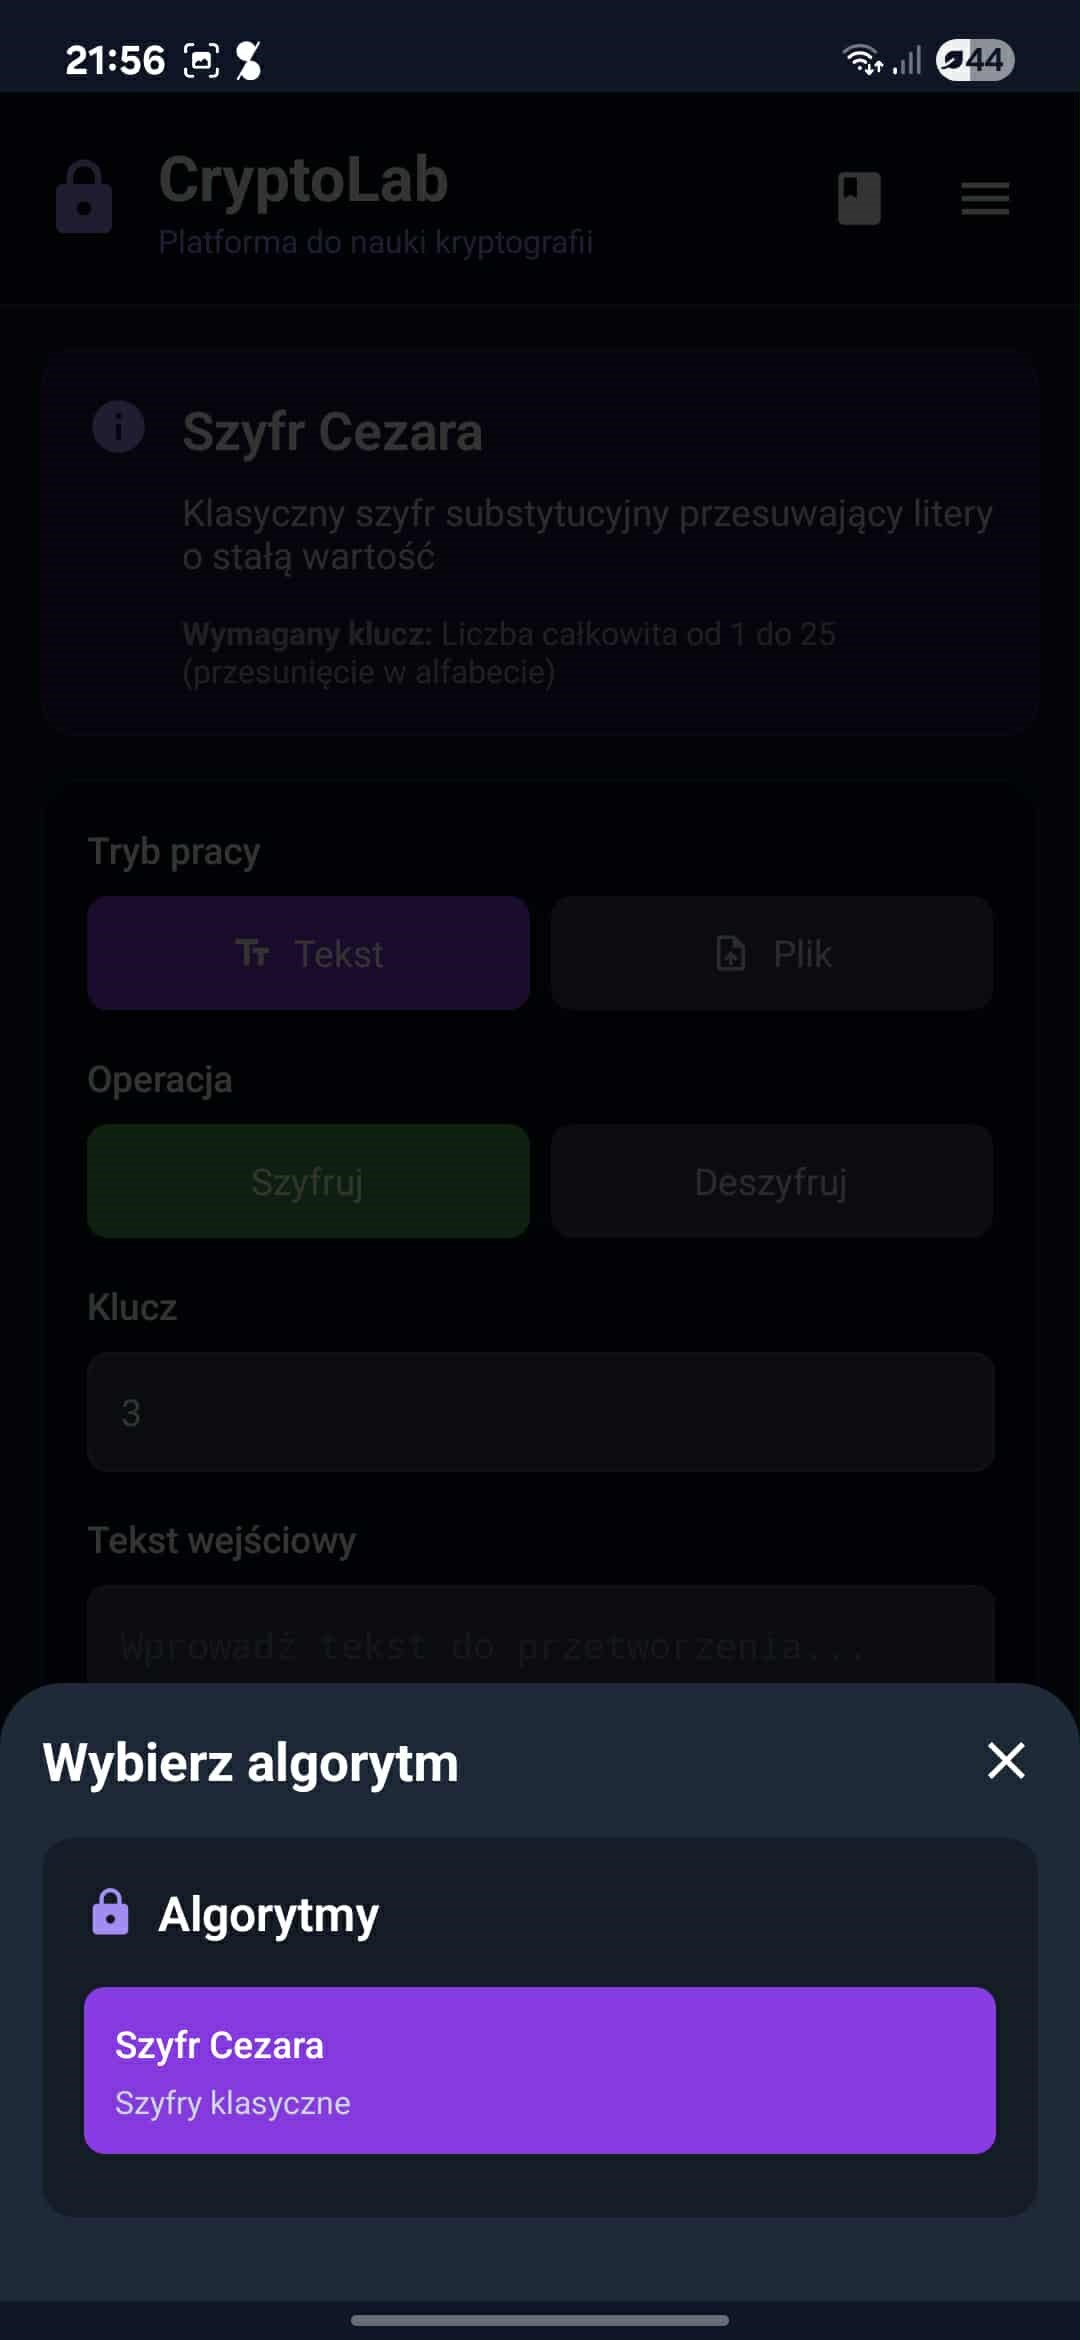
\includegraphics[width=0.3\textwidth]{img/lista_wyboru.jpg}
    \caption{Lista z możliwością wyboru algorytmu}
    \label{fig:list}
\end{figure}

Rysunek \ref{fig:main} przedstawia ekran główny aplikacji CryptoLab Mobile, a rysunek \ref{fig:list} pokazuje listę dostępnych algorytmów kryptograficznych.
\subsection{Implementacja szyfru Cezara}
\begin{lstlisting}[language=TypeScript, caption={Szczegóły implementacji CaesarCipher}]
export default class CaesarCipher extends CryptographicAlgorithm {
  constructor() {
    super(
      'Szyfr Cezara',
      'Prosty szyfr substytucyjny z przesunięciem',
      'Szyfry klasyczne'
    );
  }

  validateKey(key: string): { valid: boolean; error?: string } {
    const numKey = parseInt(key, 10);
    if (isNaN(numKey) || numKey < 1 || numKey > 25) {
      return { 
        valid: false, 
        error: 'Klucz musi być liczbą od 1 do 25' 
      };
    }
    return { valid: true };
  }

  encrypt(plaintext: string, key: string): string {
    return this._process(plaintext, parseInt(key, 10));
  }

  decrypt(ciphertext: string, key: string): string {
    const shift = 26 - (parseInt(key, 10) % 26);
    return this._process(ciphertext, shift);
  }

  private _process(text: string, shift: number): string {
    return text.split('').map(char => {
      if (/[A-Za-z]/.test(char)) {
        const base = char === char.toUpperCase() ? 65 : 97;
        return String.fromCharCode(
          (char.charCodeAt(0) - base + shift) % 26 + base
        );
      }
      return char;
    }).join('');
  }
}
\end{lstlisting}
\begin{figure}[H]
    \centering
    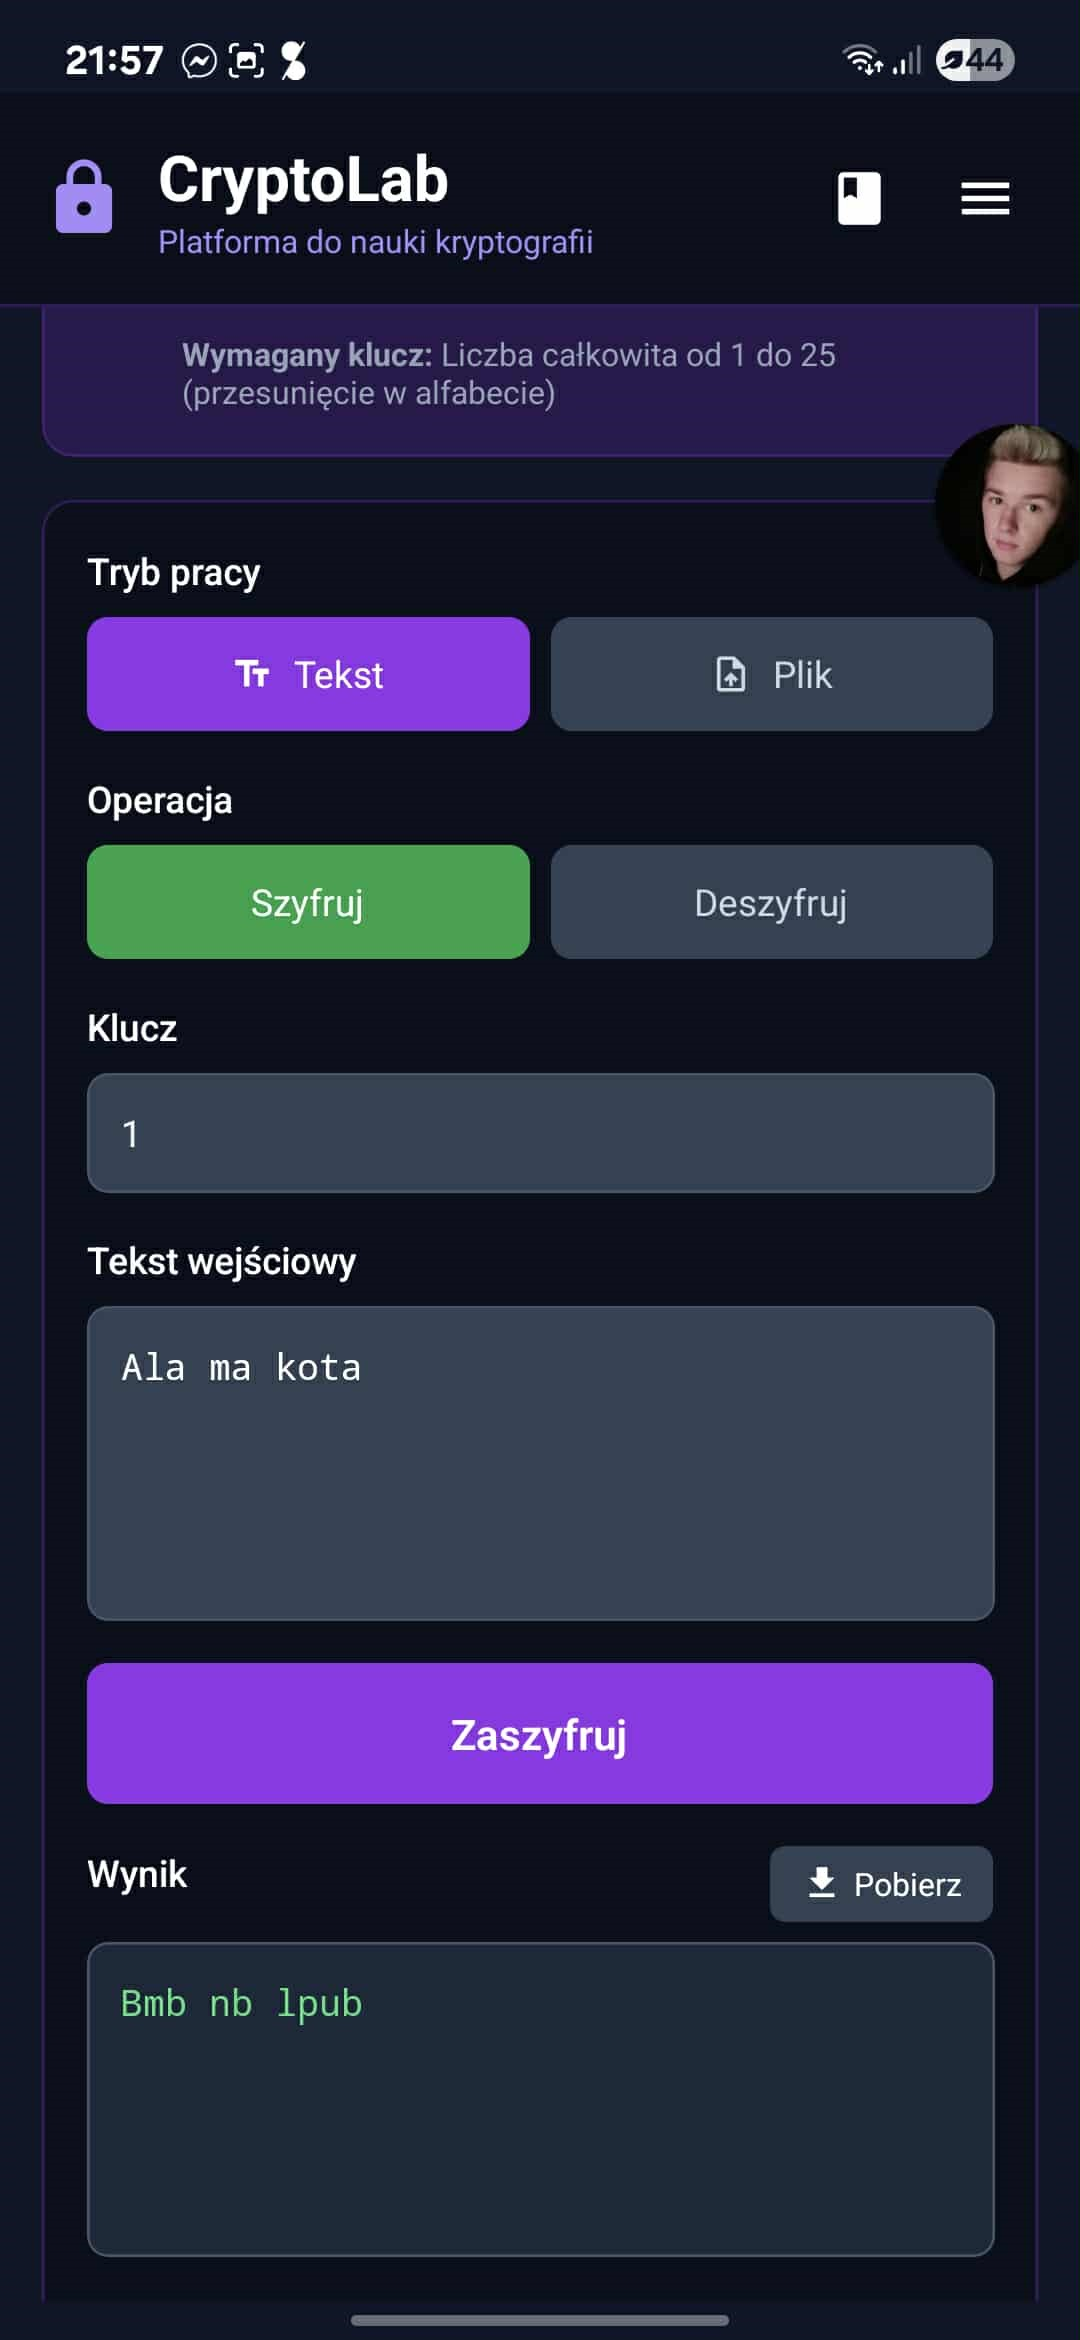
\includegraphics[width=0.3\textwidth]{img/test_cezara.jpg}
    \caption{Test szyfru Cezara}
    \label{fig:testc}
\end{figure}
Rysunek \ref{fig:testc} przedstawia przykładowy test szyfru Cezara w aplikacji CryptoLab Mobile.

\newpage
\subsection{Implementacja szyfru Vigenère'a}
\begin{lstlisting}[language=TypeScript, caption={Fragmenty klasy VigenereCipher}]
export default class VigenereCipher extends CryptographicAlgorithm {
  validateKey(key: string): { valid: boolean; error?: string } {
    if (!key || key.trim().length === 0) {
      return { valid: false, error: 'Klucz nie może być pusty' };
    }
    const hasOnlyLetters = /^[a-zA-Z]+$/.test(key);
    if (!hasOnlyLetters) {
      return { valid: false, error: 'Klucz może zawierać tylko litery' };
    }
    return { valid: true };
  }

  private _process(text: string, key: string, encrypt: boolean): string {
    let result = '';
    let keyIndex = 0;
    const normalizedKey = key.toUpperCase();
    
    for (let i = 0; i < text.length; i++) {
      const char = text[i];
      if (/[A-Za-z]/.test(char)) {
        const base = char === char.toUpperCase() ? 65 : 97;
        const textCode = char.charCodeAt(0) - base;
        const keyCode = normalizedKey.charCodeAt(keyIndex % normalizedKey.length) - 65;
        
        const resultCode = encrypt 
          ? (textCode + keyCode) % 26 
          : (textCode - keyCode + 26) % 26;
        
        result += String.fromCharCode(resultCode + base);
        keyIndex++;
      } else {
        result += char;
      }
    }
    return result;
  }
}
\end{lstlisting}

\newpage
\begin{figure}[H]
    \centering
    \includegraphics[width=0.3\textwidth]{img/szyfr_vigenerea.jpg}
    \caption{Ekran szyfru Vigenere'a}
    \label{fig:szyfrv}
\end{figure}
Rysunek \ref{fig:szyfrv} przedstawia interfejs użytkownika szyfru Vigenère'a w aplikacji CryptoLab Mobile.
\subsection{Implementacja szyfru z kluczem bieżącym}
\begin{lstlisting}[language=TypeScript, caption={Fragmenty klasy RunningKeyCipher}]
export default class RunningKeyCipher extends CryptographicAlgorithm {
  constructor() {
    super(
      'Szyfr z kluczem bieżącym',
      'Szyfr podobny do Vigenère\'a, ale używający klucza o długości tekstu',
      'Szyfry klasyczne'
    );
  }

  validateKey(key: string): { valid: boolean; error?: string } {
    if (!key || key.trim().length === 0) {
      return { valid: false, error: 'Klucz nie może być pusty' };
    }
    
    // Sprawdź czy klucz zawiera tylko litery
    const hasOnlyLetters = /^[a-zA-Z\s]+$/.test(key);
    if (!hasOnlyLetters) {
      return { valid: false, error: 'Klucz może zawierać tylko litery i spacje (A-Z, a-z)' };
    }
    
    // Policz tylko litery w kluczu
    const keyLettersCount = key.replace(/[^a-zA-Z]/g, '').length;
    if (keyLettersCount < 5) {
      return { 
        valid: false, 
        error: 'Klucz musi zawierać co najmniej 5 liter (może zawierać spacje)' 
      };
    }
    
    return { valid: true };
  }

  getKeyRequirements(): string {
    return 'Tekst (np. fragment książki) - użyto generatora lorem ipsum do stworzenia klucza';
  }
\end{lstlisting}
\begin{figure}[H]
    \centering
    \includegraphics[width=0.3\textwidth]{img/Szyfr_z_kb.jpg}
    \caption{Ekran szyfru z kluczem bieżącym}
    \label{fig:szyfrk}
\end{figure}

Rysunek \ref{fig:szyfrk} przedstawia interfejs użytkownika szyfru z kluczem bieżącym w aplikacji CryptoLab Mobile.

\newpage
\subsection{Implementacja szyfru AES}
\begin{lstlisting}[language=TypeScript, caption={Fragmenty klasy AESCipher}]
export default class AESCipher extends CryptographicAlgorithm {
  private mode: AESMode;
  public static readonly DEFAULT_KEY = '2b7e151628aed2a6abf7158809cf4f3c';

  constructor() {
    super(
      'AES (Advanced Encryption Standard)',
      'Symetryczny szyfr blokowy z możliwością wyboru trybu (ECB, CBC, CTR)',
      'Szyfry symetryczne'
    );
    this.mode = 'ECB'; // Domyślny tryb
  }

  // Ustawia tryb pracy AES
  setMode(mode: AESMode): void {
    this.mode = mode;
  }

  validateKey(key: string): { valid: boolean; error?: string } {
    if (!key || key.trim().length === 0) {
      return { valid: false, error: 'Klucz nie może być pusty' };
    }

    // Sprawdź czy klucz jest w formacie hex
    const hexPattern = /^[0-9a-fA-F]+$/;
    if (!hexPattern.test(key)) {
      return { 
        valid: false, 
        error: 'Klucz musi być ciągiem znaków szesnastkowych (0-9, A-F)' 
      };
    }

    // Klucz musi mieć długość 32, 48 lub 64 znaków hex
    if (key.length !== 32 && key.length !== 48 && key.length !== 64) {
      return {
        valid: false,
        error: 'Klucz musi mieć długość 32 (AES-128), 48 (AES-192) lub 64 (AES-256)'
      };
    }

    return { valid: true };
  }

  getKeyRequirements(): string {
    return `Tryb: ${this.mode} | Klucz hex: 32 znaki (AES-128), 
      48 (AES-192) lub 64 (AES-256)`;
  }

  // Główne metody szyfrowania wykorzystujące wybrany tryb
  encrypt(plaintext: string, key: string): string {
    if (this.mode === 'ECB') {
      return this.encryptECB(plaintext, key);
    } else if (this.mode === 'CBC') {
      return this.encryptCBC(plaintext, key);
    } else if (this.mode === 'CTR') {
      return this.encryptCTR(plaintext, key);
    }
    throw new Error(`Tryb ${this.mode} nie jest obsługiwany`);
  }
}
\end{lstlisting}

\section{Podsumowanie}

\subsection{Szyfr Cezara}
Szyfr Cezara należy do najstarszych i najprostszych technik szyfrowania. 
Jego główna idea polega na przesuwaniu liter alfabetu o ustaloną liczbę pozycji. 
Mimo że w praktyce jest to jedynie przykład historyczny, implementacja szyfru pozwala lepiej zrozumieć podstawowe mechanizmy kryptografii, takie jak klucz, szyfrowanie i deszyfrowanie.

\textbf{Zalety:}
\begin{itemize}
    \item bardzo prosta implementacja,
    \item szybkie działanie,
    \item dobre ćwiczenie dydaktyczne.
\end{itemize}

\textbf{Wady:}
\begin{itemize}
    \item niska odporność na ataki kryptograficzne,
    \item atak brute-force łatwe przełamuje szyfr w sekundach,
    \item podatny na analizę częstotliwości.
\end{itemize}

\subsection{Szyfr Vigenère'a}
Szyfr Vigenère'a to znacznie bardziej zaawansowany szyfr polialfabetyczny. 
Przez wieki uważany był za niezniszczalny, 
ale ostatecznie został przełamany dzięki analizie częstotliwości długości okresu.

\textbf{Zalety:}
\begin{itemize}
    \item znacznie bardziej bezpieczny niż szyfr Cezara,
    \item odporne na prostą analizę częstotliwości,
    \item wykorzystuje koncepcję słowa-klucza, co jest intuicyjne.
\end{itemize}

\textbf{Wady:}
\begin{itemize}
    \item niska odporność na ataki kryptograficzne (możliwy atak siłowy poprzez sprawdzenie wszystkich przesunięć),
    \item brak zastosowania we współczesnych systemach bezpieczeństwa,
    \item szyfr działa jedynie na ograniczonym zbiorze znaków (najczęściej alfabet łaciński).
\end{itemize}

\newpage
\subsection{Szyfr z kluczem bieżącym}
Szyfr z kluczem bieżącym to krok w kierunku szyfrowania jednorazowego.

\textbf{Zalety:}
\begin{itemize}
    \item gdy klucz jest losowy i używany raz -- teoretycznie nie do złamania,
    \item koncepcja zbliża się do rzeczywistego bezpieczeństwa informacyjnego,
    \item edukacyjnie pokazuje znaczenie losowości klucza.
\end{itemize}

\textbf{Wady:}
\begin{itemize}
    \item wymaga przechowywania bardzo długich kluczy,
    \item wymaga absolutnej losowości i jednorazowego użycia,
    \item niepraktyczne w większości rzeczywistych zastosowań.
\end{itemize}

\subsection{Szyfr AES}
AES (Advanced Encryption Standard) to nowoczesny szyfr symetryczny, który stanowi podstawę współczesnej kryptografii. 
W przeciwieństwie do szyfrów klasycznych, AES jest używany w realnych systemach bezpieczeństwa na całym świecie.

\textbf{Zalety:}
\begin{itemize}
    \item wysoki poziom bezpieczeństwa -- odporny na wszystkie znane praktyczne ataki,
    \item elastyczność -- obsługa trzech długości kluczy (128, 192, 256 bitów),
    \item różne tryby pracy (ECB, CBC, CTR) dostosowane do różnych zastosowań,
    \item szybkie działanie przy zachowaniu bezpieczeństwa,
    \item szeroko stosowany i przetestowany w praktyce,
    \item standaryzowany przez NIST i akceptowany globalnie.
\end{itemize}

\textbf{Wady:}
\begin{itemize}
    \item znacznie bardziej złożona implementacja niż szyfry klasyczne,
    \item wymaga zrozumienia trybów pracy i ich właściwości,
    \item tryb ECB jest niebezpieczny i nie powinien być stosowany w praktyce,
    \item wymaga bezpiecznego zarządzania kluczami i wektorami inicjalizującymi (IV),
    \item jako szyfr symetryczny, wymaga bezpiecznego przekazania klucza obu stronom komunikacji.
\end{itemize}

\textbf{Zastosowanie edukacyjne:}
\begin{itemize}
    \item pokazuje różnicę między kryptografią klasyczną a nowoczesną,
    \item wprowadza pojęcia: tryby pracy, padding, wektor inicjalizujący (IV),
    \item demonstruje znaczenie wyboru odpowiedniego trybu pracy,
    \item ilustruje jak działa rzeczywiste szyfrowanie stosowane w praktyce.
\end{itemize}


\section{Changelog}
\label{sec:changelog}
\begin{itemize}
    \item \textbf{14.10.2025} Implementacja szyfru Cezara (szyfrowanie, deszyfrowanie, walidacja klucza) oraz podstawowe GUI.
    \item \textbf{20.10.2025} Dodanie szyfru Vigenère'a i szyfru z kluczem bieżącym. \newline Ulepszenie interfejsu użytkownika. \newline 
    Implementacja AlgorithmRegistry z wzorcem Singleton. 
    \newline Ulepszenie walidacji kluczy z szczegółowymi komunikatami o błędach.
    \item \textbf{28.10.2025} Implementacja szyfru AES (Advanced Encryption Standard) z obsługą trzech trybów pracy: ECB, CBC, CTR. \newline
    Wsparcie dla kluczy AES-128, AES-192 i AES-256. \newline
    Dodanie paddingu PKCS\#7 i obsługi wektorów inicjalizujących (IV). \newline
    Pełna implementacja algorytmu AES bez użycia zewnętrznych bibliotek kryptograficznych.
\end{itemize}


\end{document}
